\documentclass[UTF8,a4paper,zihao=-4,fontset=fandol]{ctexart}
\usepackage[left=25mm,right=25mm,top=23mm,bottom=24mm]{geometry}
\usepackage{amsmath,amssymb,bm,graphicx,booktabs,longtable,array}
\usepackage{placeins,fancyhdr,xcolor,hyperref,microtype,needspace}
\definecolor{accent}{HTML}{194D68}
\hypersetup{colorlinks=true,linkcolor=accent,urlcolor=accent,pdftitle={循环MPT与CS8融合的BB码量子纠错解码技术报告},pdfauthor={钟路安}}
\setlength{\parindent}{2em}\setlength{\parskip}{0.2em}
\linespread{1.17}\setlength{\emergencystretch}{3em}
\ctexset{section={format=\Large\bfseries\color{accent}},subsection={format=\large\bfseries}}
\pagestyle{fancy}\fancyhf{}\fancyhead[L]{\small 循环MPT与CS8融合量子纠错解码}\fancyhead[R]{\small 技术报告}\fancyfoot[C]{\thepage}
\setlength{\headheight}{15pt}\renewcommand{\headrulewidth}{0.3pt}
\allowdisplaybreaks[1]
\clubpenalty=10000\widowpenalty=10000
\begin{document}
\begin{center}
{\LARGE\bfseries 面向多轮含噪测量的循环交叉注意力\\[0.25em]与有序统计融合量子纠错解码}\par
\vspace{0.7em}{\large 钟路安}\par
西安交通大学数学与统计学院\par
\vspace{0.35em}{\small AI for Science 项目技术报告\quad 2026年11月16日}
\end{center}
\vspace{0.5em}
\FloatBarrier\section*{摘要}

本研究面向BB码的12轮含噪测量，构建无辅助逻辑头的循环CrossMPT与CS8融合解码方案。模型输入两类检测事件及噪声条件，逐帧更新隐变量V、C，最终并行预测DEM故障logits，并由CS8构造满足校验的恢复。训练仅采用按期望故障数归一化的故障BCE，不使用逻辑预测损失。三个码均从随机初始化独立训练，BB72、BB90各100万样本，BB144累计600万样本，按独立验证集的故障BCE选择模型，再在新随机种子的同批样本上比较两种BP基线。


在p=0.005时，BB72、BB90各测试5000帧，BB144测试10000帧，sum-product BP+CS8错误率分别为28.34\%、15.52\%、11.65\%，循环MPT+CS8为24.18\%、11.52\%、8.33\%。相对基线的错误率降幅分别为+14.7\%、+25.8\%、+28.5\%（正值表示改善，负值表示变差）。四档噪声共12个配置中，MPT的采样错误率在12个配置低于sum-product基线。本文同时报告置信区间、配对差异及逐故障可靠性诊断，区分经验现象、充分条件与尚待验证的解释。


\textbf{关键词：}量子纠错；循环Transformer；CrossMPT；BB码；CS8；BCE。


\FloatBarrier\section{研究背景与目标}

量子信息的存储和处理受到物理噪声影响，需要通过冗余编码与反复测量校验算子来保护逻辑信息。由于测量过程本身也可能出错，单轮测量通常不足以区分数据错误与测量错误，解码器需要综合多轮记录推断恢复操作。BB码是低开销量子纠错的重要研究对象之一，其码结构和电路实现已有公开研究与工具支持。\href{https://www.nature.com/articles/s41586-024-07107-7}{Bravyi等，2024}


BP利用稀疏图进行近似概率推断，OSD则利用软信息安排代数求解与候选搜索。二者结合是量子LDPC码解码中的代表性方法。\href{https://arxiv.org/abs/2005.07016}{Roffe等，2020} 本项目关注的问题是：能否利用神经网络整合多轮测量信息，生成更有利于后处理的软信息，在保持校验约束的同时进一步降低逻辑错误率？


本文结合两个已有方向：CrossMPT利用掩码交叉注意力实现变量节点与校验节点之间的信息交换；AlphaQubit展示了通过循环网络处理量子纠错测量历史的价值。本文借鉴其结构思想，面向BB码电路噪声任务实现循环CrossMPT及故障概率输出，并与OSD组合。本文不将CrossMPT、循环Transformer或OSD本身作为原创算法。\href{https://arxiv.org/abs/2405.01033}{CrossMPT论文及官方代码}；\href{https://www.nature.com/articles/s41586-024-08148-8}{AlphaQubit论文}


本项目的主要工作包括：构建从多轮测量输入到故障软信息输出的完整模型；实现与BP共享的CS8后处理和逐帧配对评测；在三种BB码及多档噪声下验证逻辑错误率收益；分析软信息可靠性及其与代数后处理的关系。


\FloatBarrier\section{问题定义与仿真表示}

\subsection{CSS码与校验测量的基本概念}

稳定子码通过一组彼此对易的Pauli算子定义编码子空间。合法编码态具有规定的稳定子特征值；当错误与某个稳定子反对易时，该校验的特征值发生翻转。解码器利用这些变化定位错误的影响，而不是直接测量存储的逻辑量子态。


CSS码把稳定子分为只含X的校验与只含Z的校验。忽略整体相位，物理Pauli错误可写成X、Z两个二进制分量：Z型校验检测X分量，X型校验检测Z分量；Y错误同时包含这两个分量。两组校验矩阵满足\(H_XH_Z^{\mathsf T}=0\)，从而保证稳定子彼此对易。这里的物理错误分量与后文DEM电路故障坐标不同。


\begin{figure}[htbp]\centering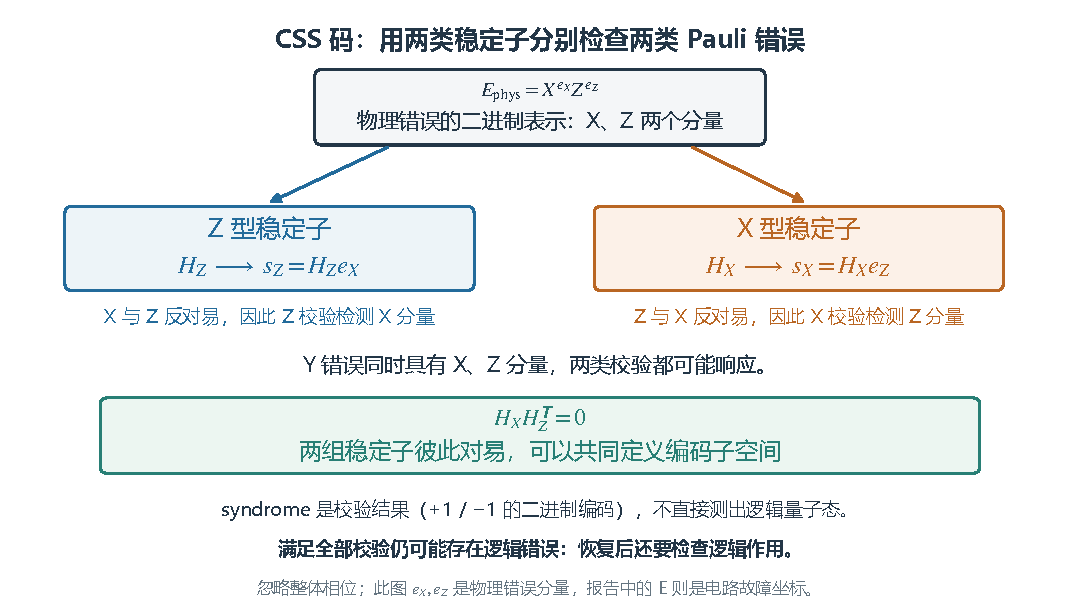
\includegraphics[width=\linewidth]{figures/css_checks_basics.pdf}\caption{CSS码的两类校验、错误分量与对易条件；此图为物理Pauli表示的概念说明}\end{figure}

以\(Z_1Z_2\)为例，可制备一个辅助比特，使两个数据比特分别控制对辅助比特的CNOT，再测量辅助比特。其结果给出\(Z_1Z_2\)的特征值，而不分别给出两个数据比特的取值。推广到更高权重稳定子时，需要与其支持集中的数据比特交互。实际含噪电路还必须规定门的调度、辅助比特复位及各位置噪声，不能由一张理想教学电路替代。


\begin{figure}[htbp]\centering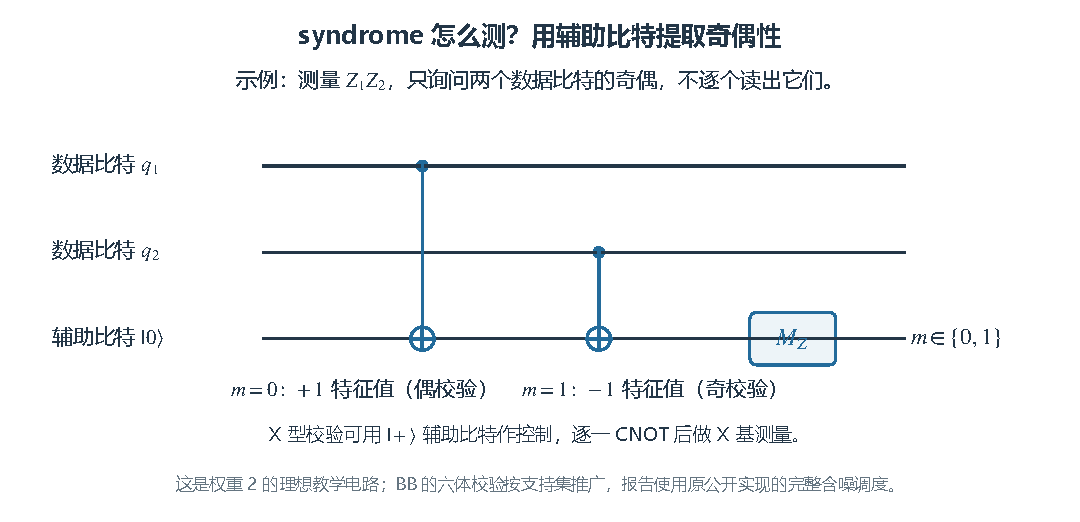
\includegraphics[width=\linewidth]{figures/stabilizer_parity_measurement.pdf}\caption{辅助比特提取Z型校验奇偶性的理想电路；BB码使用更高权重校验及完整含噪调度}\end{figure}

\subsection{BB72的结构与Tanner图表示}

BB码利用两个可交换的循环移位矩阵构造稀疏校验。本文BB72的索引参数为\(l=m=6\)，取\(A=x^3+y+y^2\)、\(B=y^3+x+x^2\)，其中x、y分别沿两个周期索引方向移位。校验矩阵为


\[
H_X=[A\;B],\qquad H_Z=[B^{\mathsf T}\;A^{\mathsf T}].
\]

由于A、B可交换，二元域上\(H_XH_Z^{\mathsf T}=AB+BA=0\)。72个数据比特可按L、R两个6\(\times\)6索引块展示，但该布局不代表实际芯片位置。每一行校验矩阵对应一个稳定子；行中非零位置就是它作用的数据比特。在Tanner图中，这表现为一个校验节点连接相应变量节点。


下图直接从发布的BB72矩阵取\(H_X\)第0行，非零位置为1、2、18、39、42、48，因此该稳定子是六个对应X算子的乘积。图中的六条连接是实际矩阵关系，不是任意绘制的示意边。网络掩码利用的正是这类校验连接结构。


\begin{figure}[htbp]\centering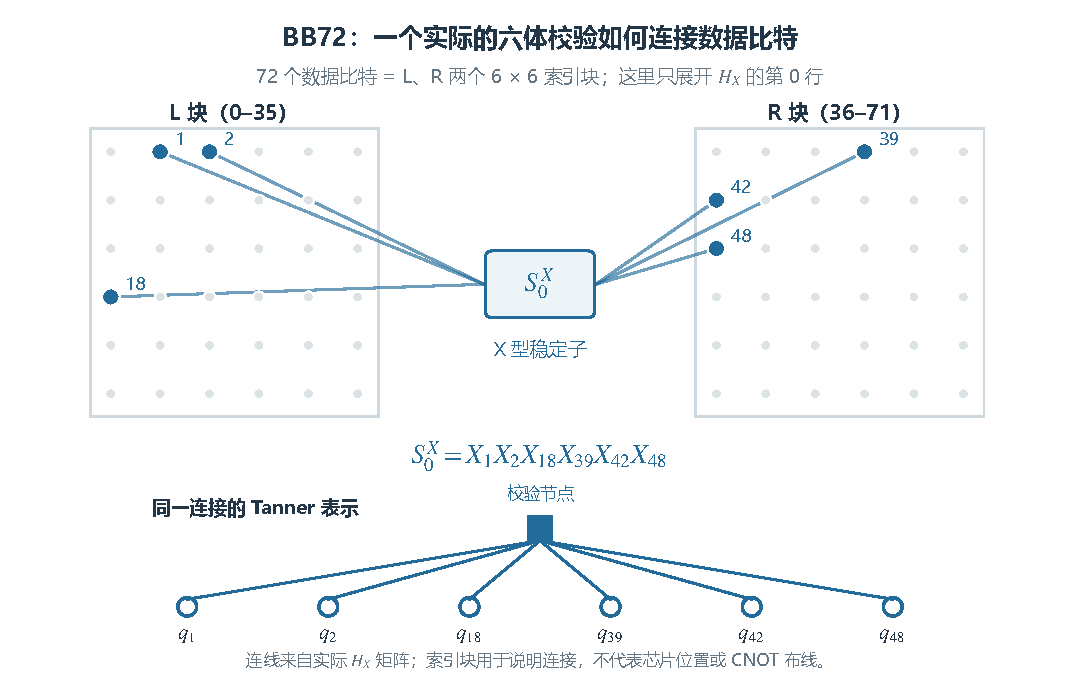
\includegraphics[width=\linewidth]{figures/bb72_check_structure.pdf}\caption{从实际BB72校验矩阵抽取的一个六体X稳定子，以及对应的Tanner连接；比特索引从0开始}\end{figure}

\subsection{多轮记忆实验}

实验采用理想初态制备和初始校验、12轮含噪校验测量、理想末轮校验及最终数据读出。相邻轮测量结果的异或形成检测事件，得到13个时间帧。这里的检测事件是二进制量；模型输入中的概率或LLR描述的是噪声条件和故障可信度，而不是将二进制测量解释为连续幅值。


仿真基于Stim，并沿用Blue等公开代码的电路生成方法。噪声覆盖公开电路中规定的单比特及双比特去极化、制备和读出等故障位置，统一由参数p控制；p是电路噪声参数，不等同于每个故障变量的概率。BB72和BB144保留公开实现的测量调度与逻辑算子；BB90使用同一电路生成流程推广，并独立验证其CSS对易关系和逻辑算子关系。\href{https://quantum-journal.org/papers/q-2021-07-06-497/}{Stim}；\href{https://quantum-journal.org/papers/q-2026-06-30-2149/}{Blue等论文}；\href{https://github.com/jblue1/ml_bb_decoding}{公开代码}


多轮测量的作用不是对随时间变化的真实syndrome进行简单多数投票。若一个数据错误在某轮出现并持续存在，受影响校验的读出可能持续翻转，差分却只在变化时刻出现；若只有单次读出被记反，通常会在该单校验时间轨迹的相邻两个差分位置出现事件。下图仅给出两种理想化轨迹，实际电路故障可能同时影响多个校验，因此需要联合时间与空间信息推断。


\begin{figure}[htbp]\centering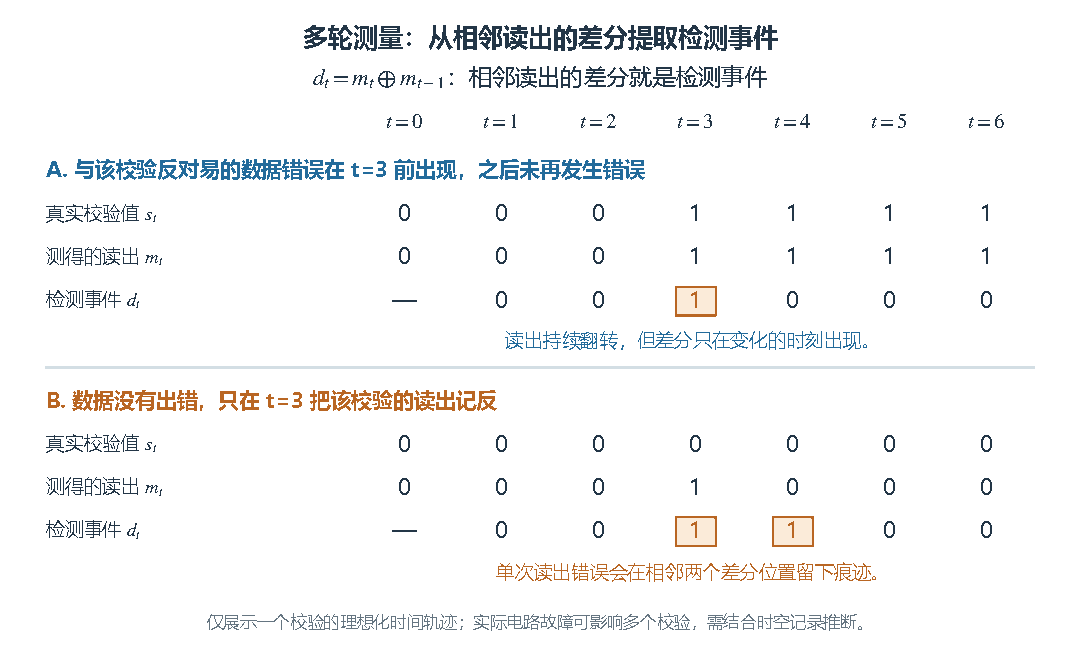
\includegraphics[width=\linewidth]{figures/syndrome_time_history.pdf}\caption{单校验时间轨迹中，持续数据错误与瞬时测量错误产生不同的检测事件模式；这是原理示意而非实验采样}\end{figure}

\subsection{故障向量、校验约束与评测目标}

在有效检测器错误模型（DEM）中，令E\(\in\)\(\mathbb F_2^N\)表示故障变量向量，H为检测事件矩阵，L为被追踪逻辑观测量的翻转映射，则


\[
s=HE,\qquad y=LE,
\]

其中运算均在二元域上进行。H的一列描述一个故障对所选检测事件的影响，L的对应列描述其对被追踪逻辑观测量的影响。具有相同检测事件和逻辑影响的有效故障合并为同一变量；这类独立DEM机制的合并概率按奇偶翻转概率计算。


解码器输出恢复向量\(\hat E\)，后处理要求


\[
H\hat E=s.
\]

本实验把所有被追踪逻辑观测量均恢复正确记为成功，即


\[
L\hat E=LE.
\]

因此，\(\hat E\)不必与E逐坐标相同。两个不同故障向量可能产生相同的检测事件和逻辑影响。本文指标为一次完整12轮记忆实验的逻辑帧错误率，不是逐故障bit错误率，也不是每轮逻辑错误率。本实验采用逻辑X记忆读出，仅评估所追踪的一组可对易逻辑观测量；不将其表述为任意未知量子态的完整纠错保真度。


\begin{table}[htbp]\centering\small\setlength{\tabcolsep}{1.6mm}\renewcommand{\arraystretch}{1.25}\begin{tabular}{@{}>{\centering\arraybackslash}p{19.66mm}>{\centering\arraybackslash}p{19.66mm}>{\centering\arraybackslash}p{19.66mm}>{\centering\arraybackslash}p{19.66mm}>{\centering\arraybackslash}p{19.66mm}>{\centering\arraybackslash}p{19.66mm}>{\centering\arraybackslash}p{19.66mm}@{}}
\toprule
\textbf{配置} & \textbf{数据比特数n} & \textbf{被追踪逻辑观测量数k} & \textbf{合并故障变量数N} & \textbf{输出H尺寸} & \textbf{rank(H)} & \textbf{模型参数量} \\
\midrule
BB72 & 72 & 12 & 4392 & 468\(\times\)4392 & 462 & 189089 \\
BB90 & 90 & 8 & 5490 & 585\(\times\)5490 & 581 & 208961 \\
BB144 & 144 & 12 & 8784 & 936\(\times\)8784 & 930 & 268577 \\
\bottomrule\end{tabular}\end{table}

N统计电路故障表示的坐标数，与物理数据比特数n不同。不同配置的n、k、故障词表及电路均不同，不能仅通过跨码错误率大小推断码结构优劣。


\FloatBarrier\section{循环MPT与CS8融合解码方法}

整体流程分为三个层次：循环部分逐帧读入测量特征并更新隐变量\(V,C\)；单帧MPT用两次有顺序的交叉注意力更新这两组隐变量；序列读完后，独立输出头把隐变量转换为全部故障的logits，再接CS8。下文分别给出三张图，避免把循环、注意力与输出头挤在同一流程中。“共享”表示时间帧之间共享参数，不表示三个BB码共用一组训练权重。


\begin{figure}[htbp]\centering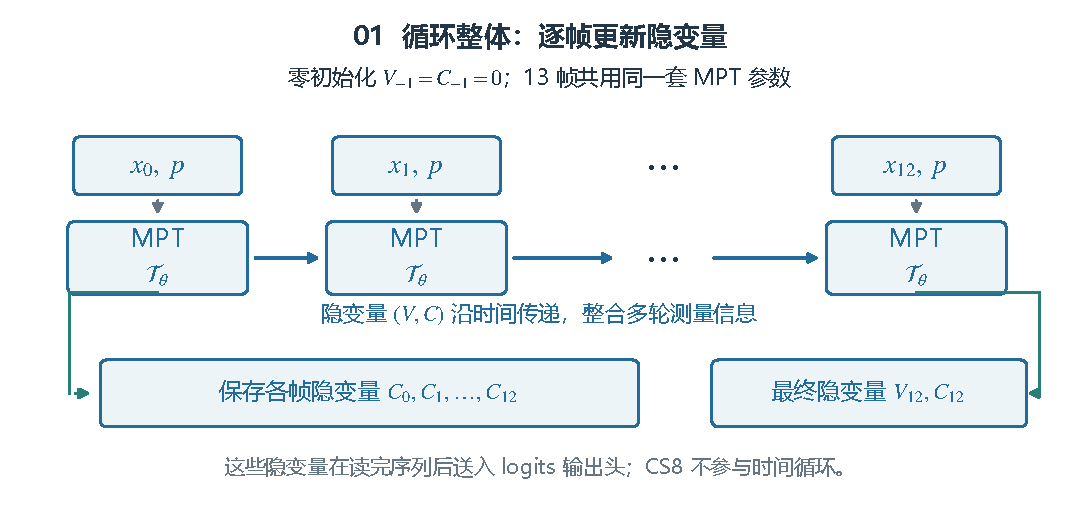
\includegraphics[width=\linewidth]{figures/model_01_recurrence.pdf}\caption{循环整体：13帧共享MPT参数，横向传递隐变量V、C。每帧C均被保存；图中仅画一条缓存支路，最终隐变量另送输出头}\end{figure}

\subsection{测量输入与噪声条件}

每个时间帧、每个校验节点使用四维特征：检测事件的累计异或值、当前检测事件、有效标记和末帧标记。当前固定长度电路中有效标记恒为1。模型同时接收两类校验的信息，输入张量形状为13\(\times\)n\(\times\)4。


此外，将噪声参数p变换为相对参考值的logit条件：


\[
c(p)=W_p\left[\operatorname{logit}(p)-\operatorname{logit}(0.003)\right].
\]

该条件分别加入隐变量\(V,C\)。当前帧测量特征的嵌入加入C。对于每个输出故障，模型还使用DEM计算得到的实际先验概率\(q_i\)。因而p与\(q_i\)承担不同功能：p提供整体电路噪声条件，\(q_i\)保留不同故障位置的非均匀先验。


\subsection{共享参数的循环交叉注意力}

模型维护两组隐变量\(V,C\)，维度均为\(n\times64\)。本文只用符号V和C称呼它们，不为每一维赋予预先规定的物理意义。按时间顺序读入13帧，每帧运行两层、四头的掩码交叉注意力。注意力的连接范围由CSS校验矩阵构造的固定掩码控制。


每一层先以归一化V为查询来源、以C为键和值的来源更新V，经过残差与FFN后，再以归一化C为查询来源、以新的V为键和值的来源更新C。Q、K、Value分别经过线性投影。同一层的两个方向复用模块参数，两层之间则有各自参数；第1层后和第2层后均对两组隐变量做LayerNorm。


\begin{figure}[htbp]\centering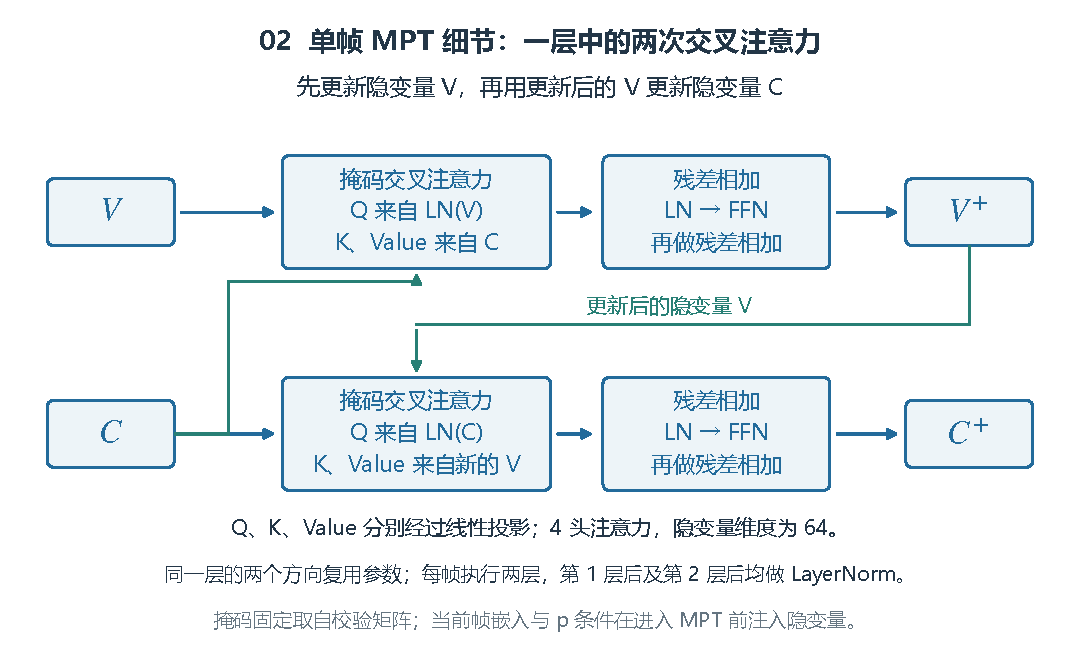
\includegraphics[width=\linewidth]{figures/model_02_mpt_layer.pdf}\caption{单帧MPT的一层细节：先更新隐变量V，再使用新的V更新隐变量C；图中LN表示LayerNorm，每帧执行两层}\end{figure}

循环更新可概括为


\[
(V_t,C_t)=\mathcal T_\theta\left(
\frac{V_{t-1}+B_V+c_V(p)}{\sqrt2},
\frac{C_{t-1}+\phi(x_t)+B_C+c_C(p)}{\sqrt2}
\right),
\]

其中B为可学习的位置嵌入，\(\phi\)为输入嵌入，\(\mathcal T_\theta\)在各时间帧共享参数。模型采用无门控循环，不使用自回归逐bit生成；全部故障概率在读完测量序列后并行输出。交叉注意力核心沿用官方CrossMPT的残差与LayerNorm组织方式，并使用GELU前馈网络。


这种设计把时间信息保存在循环传递的隐变量中，同时保留每帧C供故障输出头聚合，避免仅依赖最后一帧。


\subsection{故障概率输出与监督训练}

对每个故障i，先把各帧隐变量C投影至16维，再按该故障关联的时空位置进行平均。另一方面，对最终隐变量V和C分别取位置均值，将两个64维向量拼接并投影至16维。二者再与16维故障身份嵌入、1维相关检测事件计数及1维缩放先验logit拼接，得到50维输入。输出头为50\(\to\)32\(\to\)1的前馈网络，其输出作为先验logit的修正量：


\[
z_i=\log\frac{q_i}{1-q_i}+r_{\theta,i},\qquad
\hat p_i=\sigma(z_i).
\]

\begin{figure}[htbp]\centering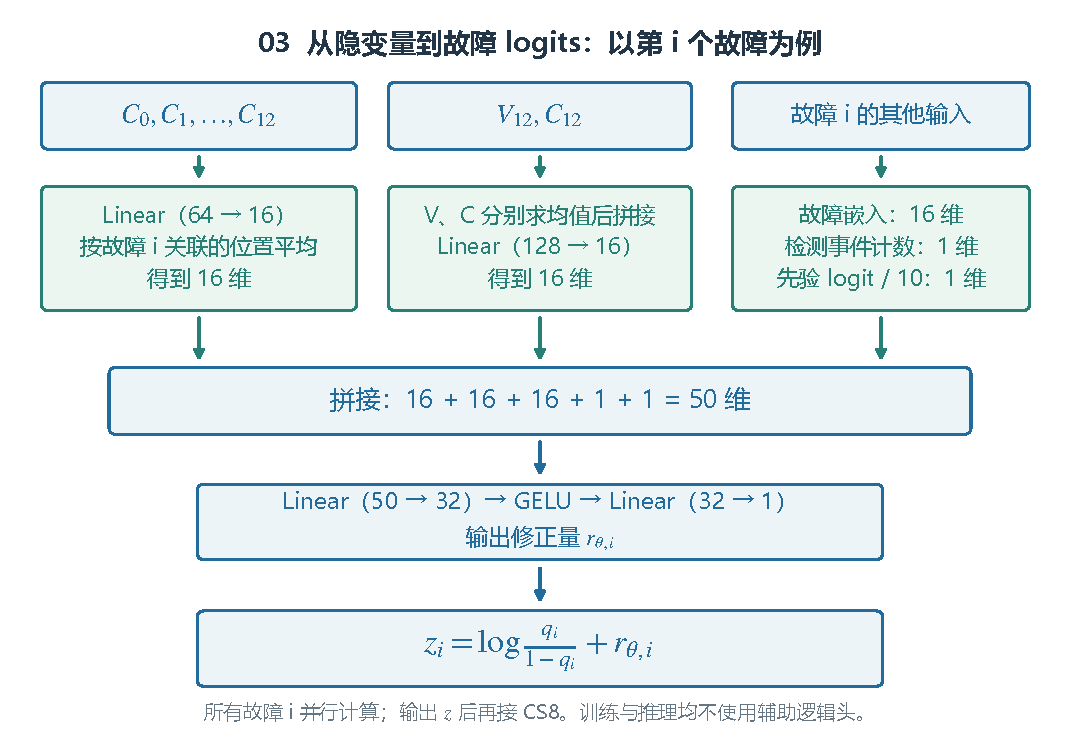
\includegraphics[width=\linewidth]{figures/model_03_logits_head.pdf}\caption{故障logits输出头：来自各帧C、最终V和C的两路16维量，与故障侧输入拼接后预测修正量；所有故障并行计算}\end{figure}

为避免符号混淆，本文统一定义


\[
\lambda_i=\log\frac{1-\hat p_i}{\hat p_i}=-z_i.
\]

硬判决为\(\hat e_i^{\rm hard}=\mathbf1[z_i>0]\)，可信度排序的诊断使用\(|\lambda_i|\)。这里\(|\lambda_i|\)较小表示边际概率接近1/2，不自动意味着模型在时间上发生震荡。


训练样本在线生成：在有效DEM中采样故障，计算完整检测事件、合并后的输出故障标签及逻辑标签。训练输入不含真实故障标签；标签仅用于监督。测试样本由Stim DEM采样器生成，真实故障记录仅用于离线评价。


训练损失仅为故障二元交叉熵，按批大小和期望故障数归一化：


\[
\mathcal L=\frac{1}{B\,\mu(p)}\sum_{b=1}^{B}\sum_{i=1}^{N}
\operatorname{BCEWithLogits}(z_{b,i},E_{b,i}),\qquad \mu(p)=\sum_iq_i.
\]

模型没有辅助逻辑预测头，不使用逻辑标签作为训练目标，也未引入OSD的可微替代损失。逻辑标签仅用于离线评价最终恢复。网络的前向接口只返回故障logits。最终模型均从头训练，不是从含辅助监督的旧权重删头或微调。


\subsection{共享的CS8后处理}

本文主实验对BP与MPT使用完全相同的后处理实现，保留已有系统的零中心构造：按\(z_i\)从大到小，即按有符号LLR \(\lambda_i\)从小到大扫描列，选取线性无关的列作为待求主元。该规则不是按\(|\lambda_i|\)排序的硬判决中心变体。


设r=rank(H)，所选r列构成集合P，其余列为自由坐标。基础候选将自由坐标设为0，通过消元求出主元部分，使H\(\hat E\)=s。CS8进一步枚举每个自由坐标的单次翻转，以及排序最前8个自由坐标的两两翻转；每次翻转均通过主元补偿维持校验约束。候选数为


\[
1+(N-r)+\binom{\min(8,N-r)}{2}.
\]

因此，“CS8”不意味着只修改8个bit，也不意味着低于某个LLR阈值的所有坐标都被纳入待求集合。选取独立列时可能跳过低LLR但线性相关的列。


主实验使用信道先验代价


\[
J_{\rm prior}(\hat E)=\sum_i\hat E_i\log\frac{1-q_i}{q_i}
\]

选择候选。该代价对应有效独立故障先验下的单个候选代价，不是对整个逻辑等价类概率求和。另保留\(J_{\rm post}(\hat E)=-\sum_i z_i\hat E_i\)的后验边际评分作为补充比较；其并非真实联合后验。主表统一使用先验评分，不按测试点挑选更优评分。各方法均关闭提前退出，以保持后处理规则一致。


\FloatBarrier\section{实验设置与可复现性}

BB72、BB90、BB144均采用无辅助头、两层四头d64循环MPT，从随机初始化独立训练，BB72、BB90各100万样本，BB144累计600万样本。训练噪声p在0.003、0.004、0.005、0.006中按相同分布抽取。训练样本由有效DEM在线生成，损失仅为故障BCE/期望故障数。AdamW，batch64，权重衰减10\(^{-4}\)，梯度裁剪1，EMA系数0.99。前10万样本采用3\(\times\)10\(^{-4}\)到3\(\times\)10\(^{-5}\)的余弦学习率，随后重置优化器，以10\(^{-4}\)起每20万样本减半、最低10\(^{-5}\)，再训练90万样本。BB144此后完整接续模型、EMA、优化器和随机数状态，分两段继续训练至400万和600万样本；后续学习率保持10\(^{-5}\)，不使用历史辅助头模型初始化。


每档噪声有1024个独立验证样本，每约10万训练样本评估一次；按四档平均归一化故障BCE最低的EMA检查点选模型。训练种子为21801115加码长。BB72、BB90执行100万样本预算，BB144执行600万样本预算；均不将达到预算上限称为完全收敛。BB144在600万时仍有验证损失下降，因资源预算暂停。


最终主表共32000帧：BB72、BB90各8000帧（p=0.005各5000帧，其余各1000帧）；BB144使用600万样本检查点冻结后的新种子测试集16000帧（p=0.005有10000帧，其余各2000帧）。每个码、每个噪声点的全部方法共享同一批样本。训练预算在探索过程中分阶段增加，最终检查点只依据固定独立验证集的故障BCE选择；最新BB144测试集未用于检查点选择。种子、模型哈希、训练记录和逐帧结果均保留。单训练种子的结果尚不量化训练方差。


min-sum与sum-product基线均使用同一单类输出检测器矩阵和非均匀DEM先验、parallel调度及最多200次迭代。min-sum配置ms\_scaling\_factor=0。全部方法使用相同的零中心有符号排序CS8、信道先验评分及关闭提前退出。BP的无穷LLR截断至\(\pm\)10\(^{6}\)，NaN回退到先验，非有限数数量有记录。神经网络输入两类检测事件，BP使用单类图，因此这里比较完整流程，不能只归因于神经网络替代BP。


无噪声电路、故障概率合并、故障到检测事件及逻辑标签的映射和每个恢复的校验一致性均被检查。代码不把DEM故障坐标的重量当作物理Pauli重量。


\FloatBarrier\section{实验结果}

\subsection{统一纯BCE训练后的逻辑错误率}

\begin{table}[htbp]\centering\small\setlength{\tabcolsep}{1.6mm}\renewcommand{\arraystretch}{1.25}\begin{tabular}{@{}>{\centering\arraybackslash}p{23.47mm}>{\centering\arraybackslash}p{23.47mm}>{\centering\arraybackslash}p{23.47mm}>{\centering\arraybackslash}p{23.47mm}>{\centering\arraybackslash}p{23.47mm}>{\centering\arraybackslash}p{23.47mm}@{}}
\toprule
\textbf{码} & \textbf{p} & \textbf{帧数} & \textbf{MS+CS8} & \textbf{SPA+CS8} & \textbf{MPT+CS8} \\
\midrule
BB72 & 0.003 & 1000 & 4.70\% & 4.80\% & 3.40\% \\
BB72 & 0.004 & 1000 & 12.70\% & 12.90\% & 11.20\% \\
BB72 & 0.005 & 5000 & 30.60\% & 28.34\% & 24.18\% \\
BB72 & 0.006 & 1000 & 55.20\% & 51.40\% & 46.80\% \\
BB90 & 0.003 & 1000 & 1.30\% & 1.30\% & 0.20\% \\
BB90 & 0.004 & 1000 & 5.10\% & 4.40\% & 2.50\% \\
BB90 & 0.005 & 5000 & 17.28\% & 15.52\% & 11.52\% \\
BB90 & 0.006 & 1000 & 38.70\% & 32.80\% & 29.10\% \\
BB144 & 0.003 & 2000 & 0.35\% & 0.35\% & 0.15\% \\
BB144 & 0.004 & 2000 & 2.55\% & 2.15\% & 1.20\% \\
BB144 & 0.005 & 10000 & 12.29\% & 11.65\% & 8.33\% \\
BB144 & 0.006 & 2000 & 37.90\% & 32.40\% & 29.15\% \\
\bottomrule\end{tabular}\end{table}

\begin{figure}[htbp]\centering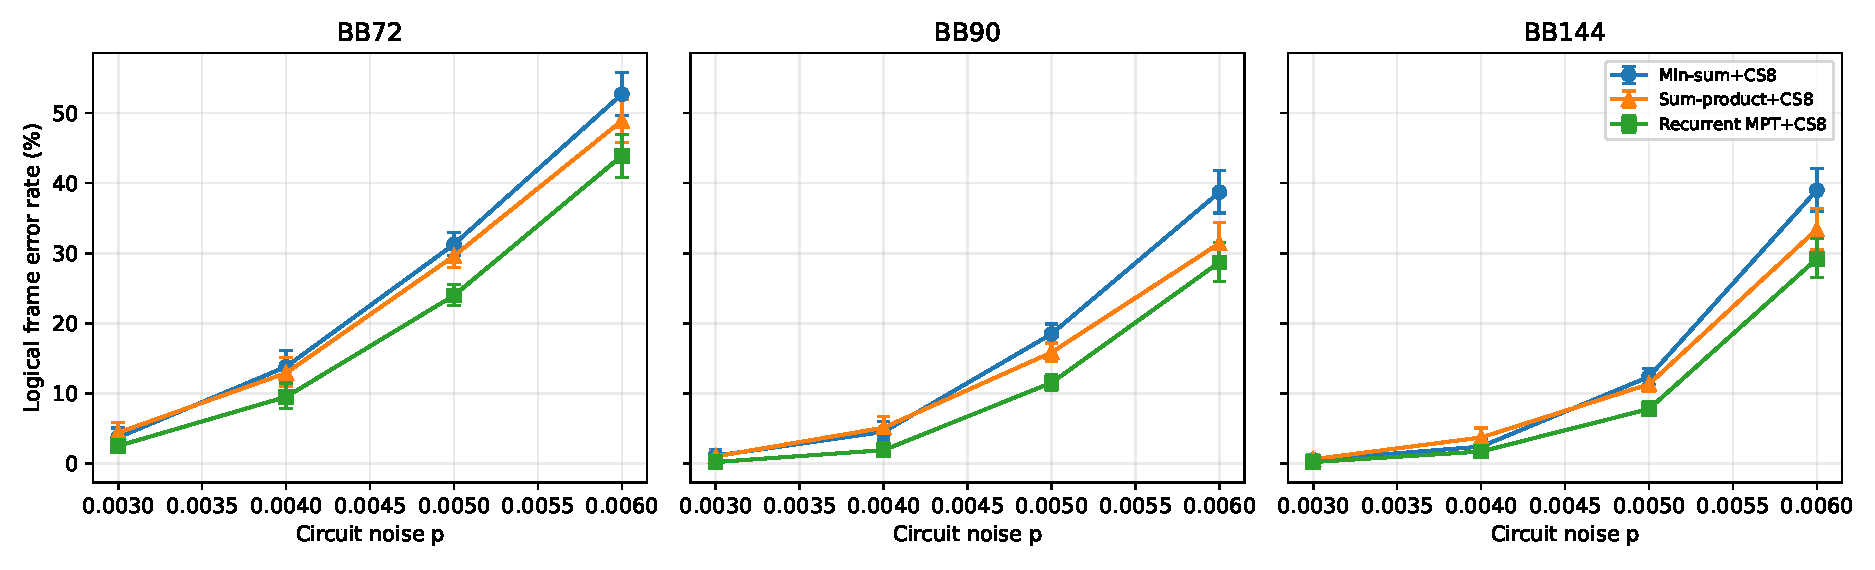
\includegraphics[width=\linewidth]{sum_product_comparison.pdf}\caption{无辅助头纯BCE模型与两种BP基线；误差棒为95\% Wilson区间}\end{figure}

\subsection{配对统计与解释}

在p=0.005，以同一测试帧上的失败差值计算成功率变化，正值表示MPT更好。下面区间为配对均值差的近似95\%区间，未对多重比较校正。


\begin{table}[htbp]\centering\small\setlength{\tabcolsep}{1.6mm}\renewcommand{\arraystretch}{1.25}\begin{tabular}{@{}>{\centering\arraybackslash}p{36.80mm}>{\centering\arraybackslash}p{36.80mm}>{\centering\arraybackslash}p{36.80mm}>{\centering\arraybackslash}p{36.80mm}@{}}
\toprule
\textbf{码} & \textbf{成功率变化} & \textbf{配对95\%区间} & \textbf{错误率相对降幅} \\
\midrule
BB72 & +4.16个百分点 & [+3.03,+5.29]个百分点 & +14.7\% \\
BB90 & +4.00个百分点 & [+2.97,+5.03]个百分点 & +25.8\% \\
BB144 & +3.32个百分点 & [+2.66,+3.98]个百分点 & +28.5\% \\
\bottomrule\end{tabular}\end{table}

是否支持明确改善应结合配对区间是否跨0、样本量及单训练种子的限制判断。这里没有在新旧模型之间按测试结果挑选，也未将历史含辅助头模型的成绩混入新主表。


\subsection{BB144训练预算与验证进展}

BB144从头训练后，固定验证集的平均归一化故障BCE在100万、400万、600万样本时分别为1.7280、1.6438、1.6153，未见验证损失持续回升。以下为最终同一新测试集上的阶段对比，仅作训练进展诊断，不据此重新挑选检查点：


\begin{table}[htbp]\centering\small\setlength{\tabcolsep}{1.6mm}\renewcommand{\arraystretch}{1.25}\begin{tabular}{@{}>{\centering\arraybackslash}p{28.80mm}>{\centering\arraybackslash}p{28.80mm}>{\centering\arraybackslash}p{28.80mm}>{\centering\arraybackslash}p{28.80mm}>{\centering\arraybackslash}p{28.80mm}@{}}
\toprule
\textbf{p} & \textbf{帧数} & \textbf{100万版} & \textbf{400万版} & \textbf{600万版} \\
\midrule
0.003 & 2000 & 0.20\% & 0.15\% & 0.15\% \\
0.004 & 2000 & 1.50\% & 1.45\% & 1.20\% \\
0.005 & 10000 & 10.09\% & 8.58\% & 8.33\% \\
0.006 & 2000 & 34.45\% & 30.65\% & 29.15\% \\
\bottomrule\end{tabular}\end{table}

600万版相较400万版，在p=0.005改善0.25个百分点，配对区间仍跨0；在p=0.006改善1.50个百分点，配对区间约为[0.38,2.62]个百分点。该结果说明延长训练可以改善本模型，但不意味着误差率随每次验证损失下降而单调降低，也不构成辅助逻辑监督作用的受控消融。阶段对比与逐帧输出另见训练进展补充材料。


\begin{figure}[htbp]\centering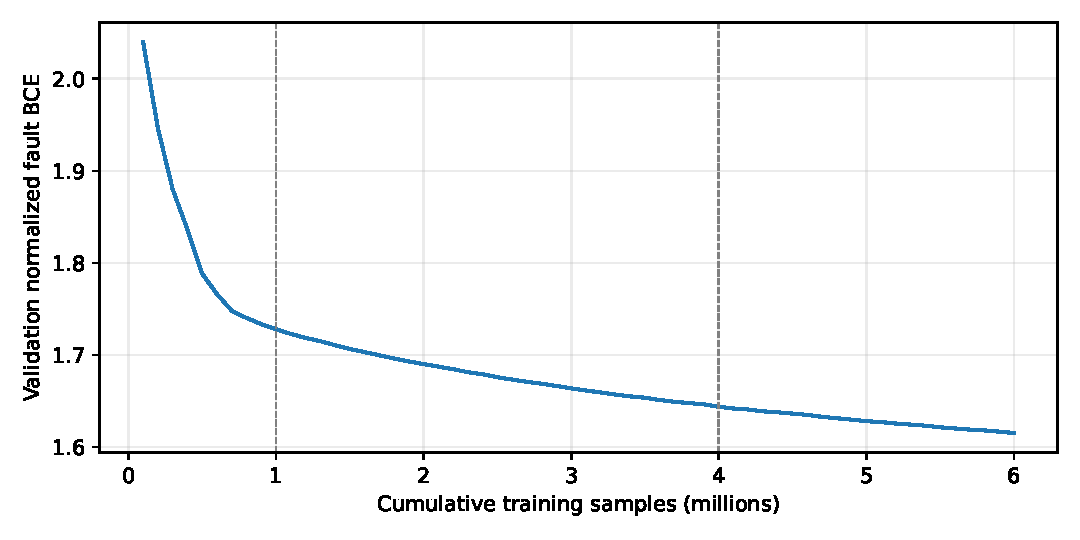
\includegraphics[width=\linewidth]{training_progress.pdf}\caption{BB144固定验证集的训练进展；虚线标记100万与400万样本}\end{figure}

\FloatBarrier\section{可靠性分析与后处理的改进空间}

\subsection{软信息排序与保留部分的可靠性}

分别按各模型的绝对LLR排序，释放C个最不确定坐标，统计其余固定硬判决与真实故障表示的差异t(C)。相同C意味着同一码内固定坐标数相同，但各模型选择的集合不同。该诊断比较可靠性排序，不是同一数值阈值下的概率校准，也不是主表有符号排序CS8的精确复现。


\begin{table}[htbp]\centering\small\setlength{\tabcolsep}{1.6mm}\renewcommand{\arraystretch}{1.25}\begin{tabular}{@{}>{\centering\arraybackslash}p{28.80mm}>{\centering\arraybackslash}p{28.80mm}>{\centering\arraybackslash}p{28.80mm}>{\centering\arraybackslash}p{28.80mm}>{\centering\arraybackslash}p{28.80mm}@{}}
\toprule
\textbf{码} & \textbf{C} & \textbf{MPT平均t} & \textbf{Min-sum平均t} & \textbf{Sum-product平均t} \\
\midrule
BB72 & 32 & 9.06 & 9.59 & 8.00 \\
BB72 & 128 & 3.04 & 6.56 & 5.62 \\
BB72 & 512 & 0.62 & 4.43 & 3.92 \\
BB90 & 32 & 12.58 & 11.95 & 10.31 \\
BB90 & 128 & 4.64 & 8.45 & 7.46 \\
BB90 & 512 & 1.05 & 5.91 & 5.33 \\
BB144 & 32 & 22.11 & 19.36 & 17.52 \\
BB144 & 128 & 9.38 & 14.80 & 13.66 \\
BB144 & 512 & 2.35 & 11.32 & 10.52 \\
\bottomrule\end{tabular}\end{table}

\begin{figure}[htbp]\centering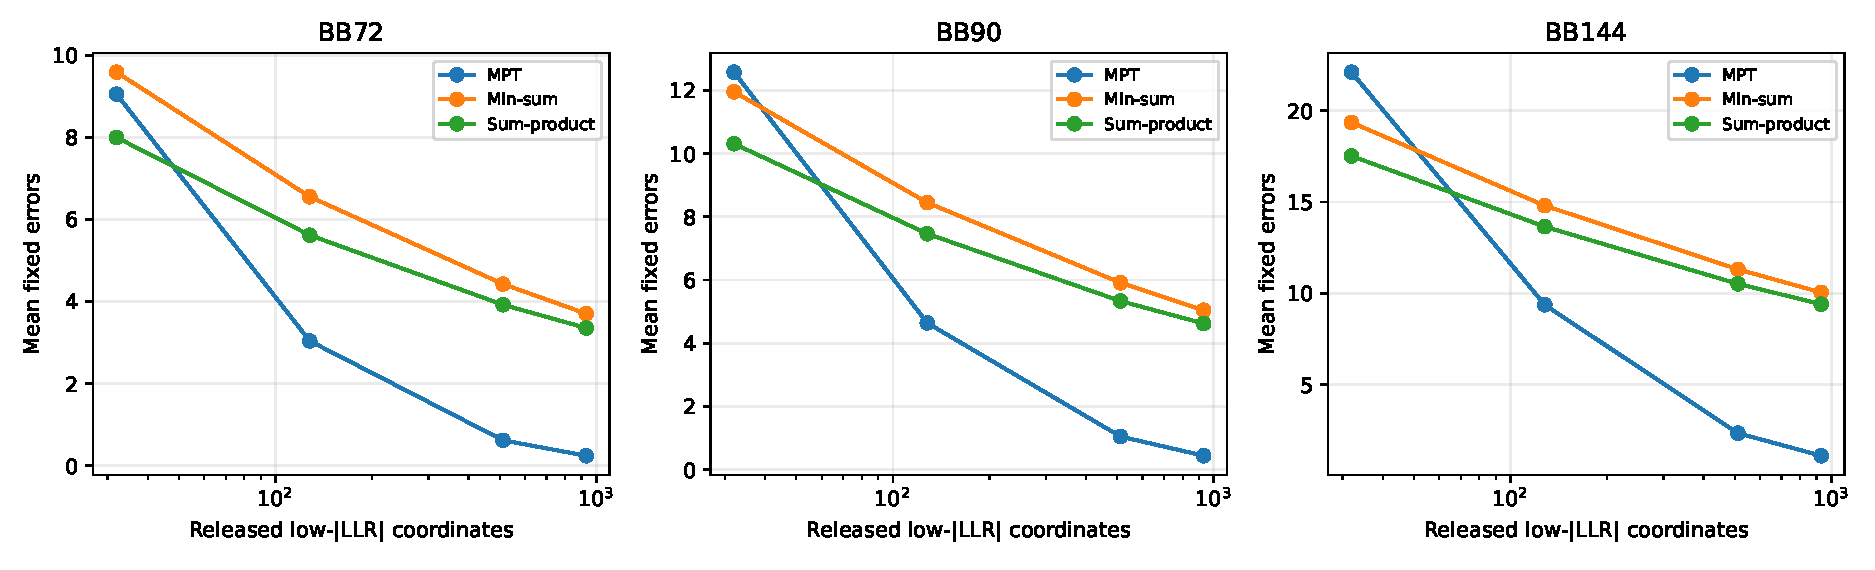
\includegraphics[width=\linewidth]{confidence_retention.pdf}\caption{p=0.005下，同等释放数对应的固定部分平均错误数}\end{figure}

上表给出本轮最终模型的实际诊断。不能由某一释放数的优势推出所有高置信度范围均有优势，也不能由平均错误数替代逐帧无错概率。可靠性排序的差异是理解后处理收益的一条线索，但输入范围、候选构造和评分也有影响，目前未将其隔离为唯一原因。


\subsection{通过小支撑线性求解控制残余重量的思路}

进一步考虑一种面向可靠性分布的后处理：把高置信度集合F的硬判决固定，仅在低置信度集合P上求解


\[
H_P\hat E_P=s\oplus H_F\hat e_F^{\rm hard}.
\]

若得到合法恢复，令\(\Delta=E\oplus\hat E\)，则\(H\Delta=0\)。设固定部分误判数为t，P中的坐标数为C，则严格有


\[
\operatorname{wt}(\Delta)
=t+\operatorname{wt}(E_P\oplus\hat E_P)
\le t+C.
\]

对于物理Pauli错误表示，如果已确认\(\Delta\)与全部稳定子对易，且物理Pauli重量小于码距，则\(\Delta\)不可能是非平凡逻辑算子，只能属于稳定子群。这正是“利用校验约束限制残余类型，再利用小重量排除逻辑错误”的数学出发点。


但是本文E是电路故障表示，不能把其重量直接与物理码距比较。应对当前H、L定义


\[
d_{\mathrm{circ},L}=\min\{\operatorname{wt}(v):Hv=0,\ Lv\ne0\}.
\]

于是有一个与本实验目标相匹配的充分条件：


\[
\boxed{H\hat E=s,\quad t+C<d_{\mathrm{circ},L}
\quad\Longrightarrow\quad L\hat E=LE.}
\]

该结论不需要唯一识别真实故障，只要求残余不能产生被追踪的逻辑翻转。它是条件保证，并不说明我们的算法已满足条件：当前尚未获得该距离的可靠下界，t也不能在实际推理时由未知真值直接计算。平均t较小更不能代替逐帧尾概率控制。


“小支撑”也不等同于“小秩”。若|P|小于rank(H)，右侧可能不在\(H_P\)的列空间中，方程没有解；若\(H_P\)存在非零核，即使方程有解，满足校验的多个候选仍可能有不同逻辑作用。因此，释放坐标数、子矩阵秩、核空间逻辑作用和候选选择需要共同考虑。


两个更直接的代数条件是：若F全部正确且\(H_P\)满列秩，则真实E\_P是唯一解；若F全部正确，且对所有v\(\in\)ker(\(H_P\))均有\(L_P\)v=0，则即使解不唯一，所有解也具有相同的被追踪逻辑标签。这些条件提示了比单纯放大待求集合更有针对性的结构分析方向，但本文未把它们实现为新的、已验证有效的解码器。


\subsection{与BP+OSD的联系及尚未解决的问题}

上述思路与BP+OSD具有共同直觉：先用概率信息缩小不确定性，再通过代数求解使恢复满足校验，同时通过候选评分避免代价过大的恢复。BP改善软信息，OSD弥补独立硬判决可能违反校验的问题，两者具有互补性。


但不能据此把“残余重量必然小于距离”当作BP+OSD有效或广泛使用的已证明原因。OSD的代价函数作用于恢复候选，其并不知道真实E，因此不会直接最小化wt(E\(\oplus\)\(\hat E\))。满足校验也只说明残余位于核空间，尚未保证其逻辑作用为零。


同样，增大P虽然不会增加固定部分错误t，却会使上界t+C不减：每释放一个坐标，t最多减少1，而C增加1。该上界通常较松，不能仅靠释放更多坐标来获得更强保证。未来更值得研究的是：如何识别危险的固定错误、如何在可行解集合中选取合适恢复，以及如何利用\(H_P\)核空间的逻辑结构。


因此，当前CS8是一种有效且可复现的后处理选择，但没有证据表明它已充分利用MPT的可靠性分布，也没有最优性保证。面向MPT软信息的后处理应作为后续研究方向，不能将尚未实现的低秩方案写成本文既有成果。


\FloatBarrier\section{适用范围与研究局限}

结果限于三种BB码、固定12轮测量及所采用的电路与有效DEM。未验证真实硬件、泄漏、丢失或噪声漂移，也不声称可直接推广到任意轮数。三个码各自训练，没有共享权重的跨码泛化实验。


训练和验证、测试随机种子分离，检查点仅依据验证故障BCE选择；但目前每码仍只有一个训练种子，未量化训练波动。三个码训练预算不同，不能把跨码差异解释为单一结构因素；探索中的旧评测曾用于决定是否延长预算，最终BB144另用新测试集。误差区间主要反映有限测试帧的采样不确定性。


基线是明确配置的单类min-sum和sum-product BP+CS8，没有穷尽调度、迭代预算及其他增强BP方法。MPT使用两类检测事件，基线只使用所选单类图，输入信息范围不同。


评测只跟踪一组可对易逻辑观测量，不是完整任意量子态的逻辑信道保真度。此前BB72速度测量属于独立实验，不能直接当作本轮三个最终模型的速度结果；本文不作通用实时性或硬件无关速度优势声明。


\FloatBarrier\Needspace{70mm}\section{结论}

本轮统一采用无辅助逻辑头、仅故障BCE监督的循环CrossMPT，独立从头训练三种BB码后，在四档噪声及新测试样本上比较相同CS8流程。p=0.005时，MPT的逻辑错误率分别为24.18\%、11.52\%、8.33\%，sum-product基线为28.34\%、15.52\%、11.65\%。相对错误率降幅为+14.7\%、+25.8\%、+28.5\%。这些是单训练种子下的实验结果，统计解释以配对区间为准。


该实现直接围绕故障软信息和代数恢复构建，不依赖尚未明确验证作用的辅助逻辑监督。下一步可研究如何利用软信息分布选择可行恢复，并通过多训练种子和更广泛噪声测试评估稳定性。


\FloatBarrier\section*{参考文献与代码来源}

\noindent 1. \href{https://www.nature.com/articles/s41586-024-07107-7}{Bravyi et al. High-threshold and low-overhead fault-tolerant quantum memory. Nature, 2024.}\par\smallskip

\noindent 2. \href{https://arxiv.org/abs/2405.01033}{CrossMPT: Cross-attention Message-Passing Transformer for Error Correcting Codes. ICLR 2025.} \href{https://github.com/iil-postech/crossmpt}{官方代码}\par\smallskip

\noindent 3. \href{https://www.nature.com/articles/s41586-024-08148-8}{Bausch et al. Learning high-accuracy error decoding for quantum processors. Nature, 2024.}\par\smallskip

\noindent 4. \href{https://arxiv.org/abs/2005.07016}{Roffe et al. Decoding Across the Quantum LDPC Code Landscape. Physical Review Research, 2020.}\par\smallskip

\noindent 5. \href{https://quantum-journal.org/papers/q-2021-07-06-497/}{Gidney. Stim: a fast stabilizer circuit simulator. Quantum, 2021.}\par\smallskip

\noindent 6. \href{https://quantum-journal.org/papers/q-2026-06-30-2149/}{Blue et al. Machine Learning Decoding of Circuit-Level Noise for Bivariate Bicycle Codes. Quantum, 2026.} \href{https://github.com/jblue1/ml_bb_decoding}{电路代码}\par\smallskip
\end{document}
